\section{Neural Path Framework For CNN}\label{sec:cnpf}
\textbf{Indexing:} The weights of layers $l\in[\dc]$ are denoted by $\Theta(\icin,\iin,\iout,l)$ and for layers $l\in[\dfc]+\dc$ are denoted by $\Theta(\iin,\iout,l)$. The pre-activations, gating and hidden unit outputs are denoted by $q_{x,\Theta}(\ifout,\iout,l)$,  $G_{x,\Theta}(\ifout,\iout,l)$, and $z_{x,\Theta}(\ifout,\iout,l)$ for layers $l=1,\ldots, \dc$. $\iin$ and $\iout$ are used to index the input and the output filters. $\ifout$ is used to denote the index of hidden unit (in the feature dimension) within the input and output filters. %Here, $\icin\in[\wconv]$, for $l=1\ldots,\dc$, $\iin\in[w]$ for $l=\dc+2,\ldots,\dc+\dfc+1$, $\ifin \in[1]$ for $l=1$, $\ifin \in[w]$ for $l=2,\ldots,\dc$, $\iout\in[w]$ for $l=1\ldots,\dc, \dc+2,\ldots, \dc+\dfc$,  $\iout\in[1]$ for $l=\dc+\dfc+1$, $\ifout\in[w]$ for $l=1,\ldots,\dc$.
\begin{comment}
\FloatBarrier
\begin{table}[h]
\centering
\begin{tabular}{|c|ll|}\hline
Index & Range&\\\hline
\multirow{2}{*}{$\iin$} & $\in[\din]$ & for $l=1\ldots,\dc$\\ \cline{2-3}
&$\in[w]$ & for $l=\dc+2,\ldots,\dc+\dfc+1$\\ \hline
\multirow{2}{*}{$\ifin$} & $\in[1]$ & for $l=1$\\ \cline{2-3}
&$\in[w]$ &for $l=2,\ldots,\dc$\\ \hline
\multirow{2}{*}{$\iout$} & $\in[w]$ &for $l=1\ldots,\dc, \dc+2,\ldots, \dc+\dfc$\\ \cline{2-3}
&$\in[1]$ &for $l=\dc+\dfc+1$\\ \hline
{$\ifout$} & $\in[w]$ &for $l=1,\ldots,\dc$\\ \hline
\end{tabular}
\end{table}
\end{comment}

\textbf{Shapes:} \Cref{fig:shape-main} shows the shapes of the tensors in the convolutional layers of a $1$-dimensional circular CNN considered in this paper. Here, the input is a $1$-dimensional tensor given by $x\in\R^{\din}$. The hidden nodes in a given convolutional layer have a $2$-dimensional shape of $\din\times w$, where $w$ is the number of filters in the layer. The weights of a given convolutional layer have $3$-dimensional shape of $\wconv\times w\times w$,  where $w\times w$ is because of the number of input filters times the number of output filters.
\FloatBarrier
\begin{figure}[h]
\centering
%\resizebox{\columnwidth}{!}{
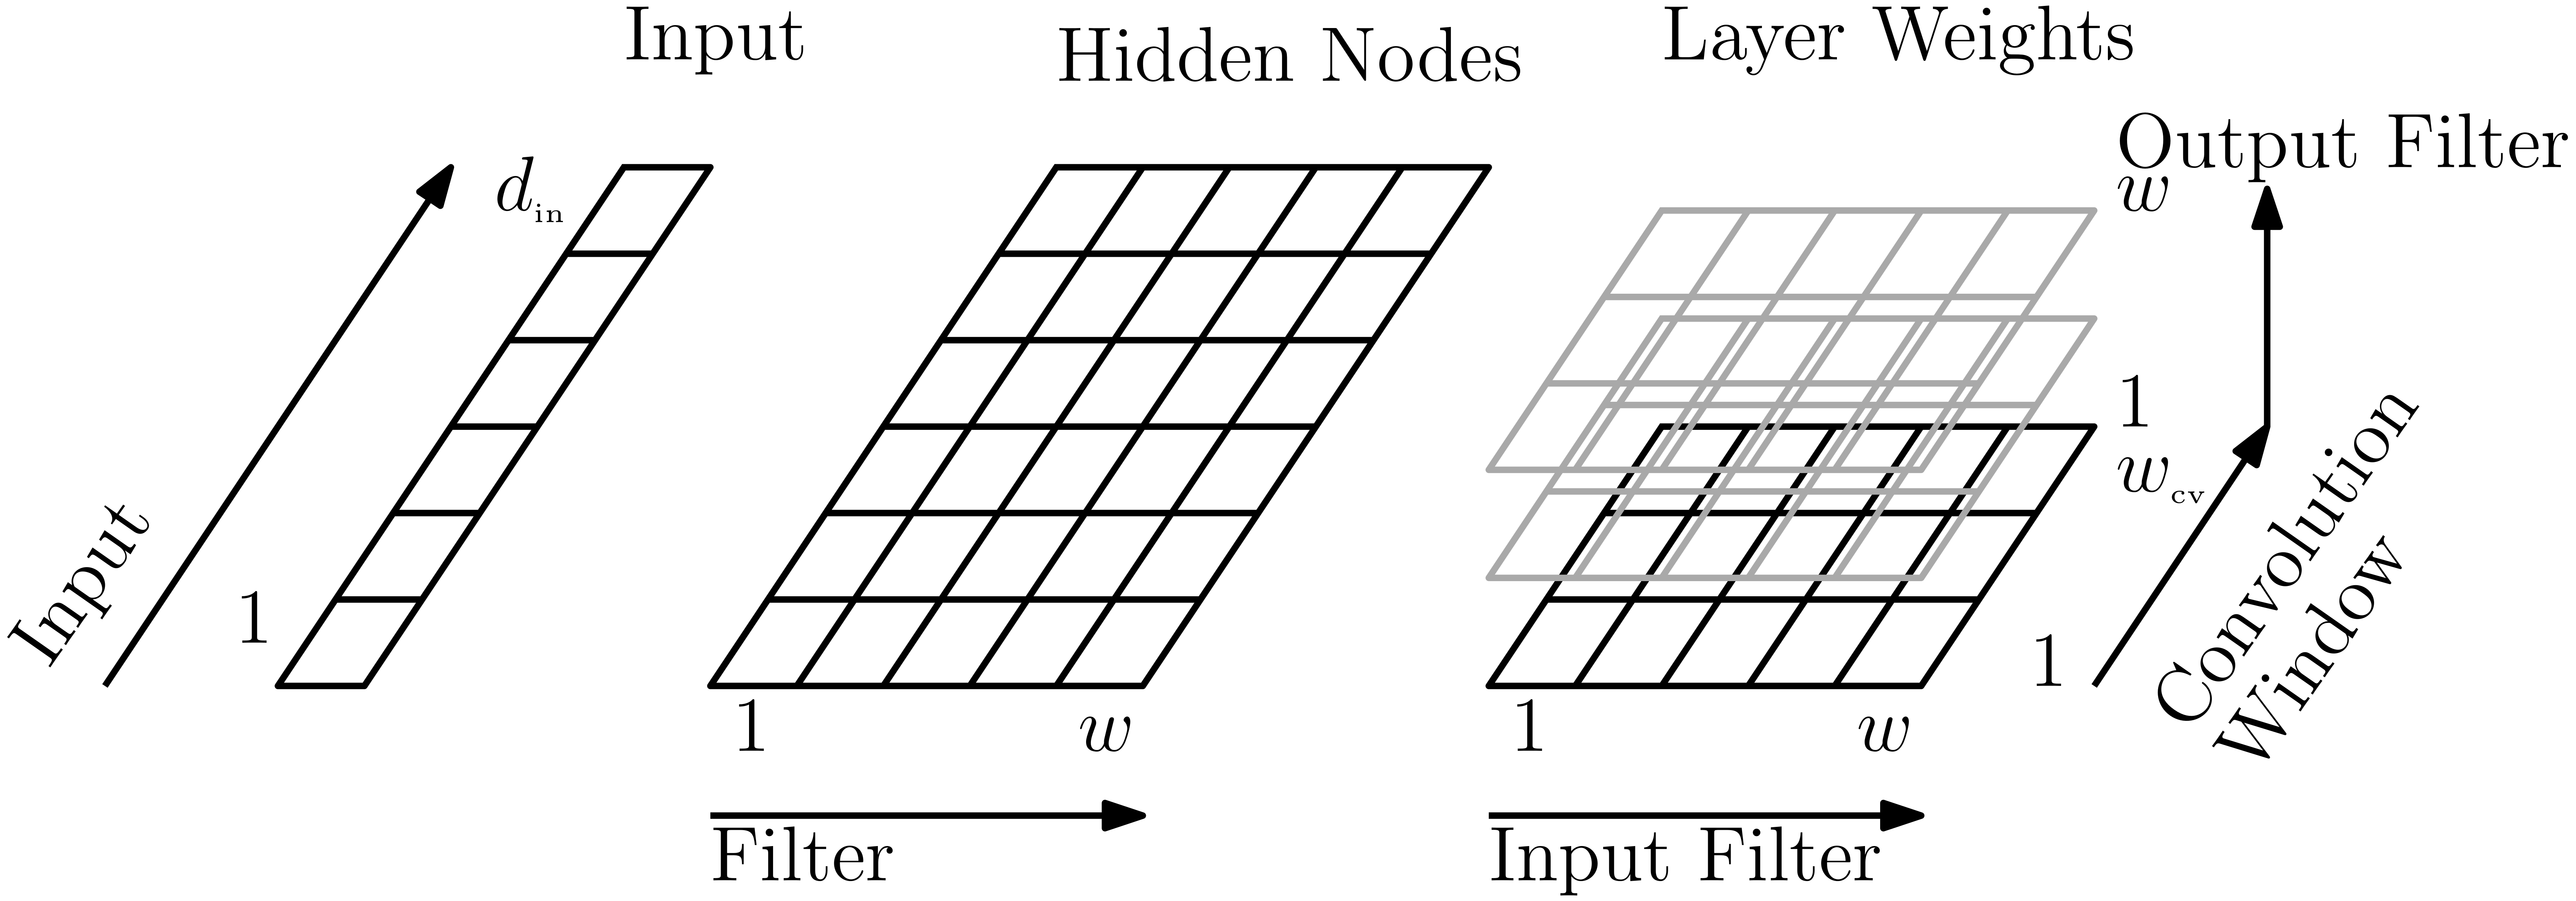
\includegraphics[scale=0.04]{figs/shape.png}
%}
\label{fig:shape-main}
\caption{Shows the shape of the tensor.}
\end{figure}

\subsubsection{Information Flow}
\begin{table}[h]
\centering
\begin{tabular}{|c l lll|}\hline
IL&: &$z_{x,\Theta}(\cdot,1,0)$ &$=$ &$x$ \\\hline\hline
\multicolumn{5}{|l|}{Convolutional Layers, $l\in[\dc]$}\\\hline\hline
PA&: & $q_{x,\Theta}(\ifout,\iout,l)$& $=$ & $\sum_{\icin,\iin}\Theta(\icin,\iin,\iout,l)\cdot z_{x,\Theta}(\ifout\oplus (\icin-1),\iin,l-1)$\\
GV&: &$G_{x,\Theta}(\ifout,\iout,l)$& $=$ & $\mathbf{1}_{\{q_{x,\Theta}(\ifout,\iout,l)>0\}}$\\
HUO&: &$z_{x,\Theta}(\ifout,\iout,l)$ & $=$ & $q_{x,\Theta}(\ifout,\iout,l)\cdot G_{x,\Theta}(\ifout,\iout,l)$\\\hline\hline
\multicolumn{5}{|l|}{GAP Layers, $l=\dc+1$}\\\hline\hline
%HUO&: &${z}_{x,\Theta}(\iout,l)$ & $=$ & $\frac{1}{\din}\sum_{i\in [\din]} z_{x,\Theta}(i,\iout,l-1)$\\\hline\hline
HUO&: &$z_{x,\Theta}(\iout, \dc+1)$ & $=$ &$\sum_{\ifout} z_{x,\Theta}(\ifout,\iout,\dc)\cdot G^{\text{pool}}_{x,\Theta}(\ifout,\iout,\dc+1)$\\\hline\hline
\multicolumn{5}{|l|}{Fully Connected Layers, $l\in[\dfc]+(\dc+1)$}\\\hline\hline
PA&: & $q_{x,\Theta}(\iout,l)$& $=$ & $\sum_{\iin}\Theta(\iin,\iout,l) \cdot z_{x,\Theta}(\iin,l-1) $\\
GV&: &$G_{x,\Theta}(\iout,l)$& $=$ & $\mathbf{1}_{\{(q_{x,\Theta}(\iout,l))>0\}}$\\
HUO&: &$z_{x,\Theta}(\iout,l)$ & $=$ & $q_{x,\Theta}(\iout,l)\cdot G_{x,\Theta}(\iout,l)$\\
FO&: & $\hat{y}_{\Theta}(x)$ & $=$ & $\sum_{\iin}\Theta(\iin,\iout, d)\cdot z_{x,\Theta}(\iin,d-1)$\\\hline
\end{tabular}
\caption{Here IL, PA, GV, HUO, GL and FO are abbreviations for input layer, pre-activation, gating values, hidden unit output, GAP-layer and final output respectively.}
\label{tb:cconv}
\end{table}

\FloatBarrier
\begin{figure}[H]
\centering
\resizebox{\columnwidth}{!}{
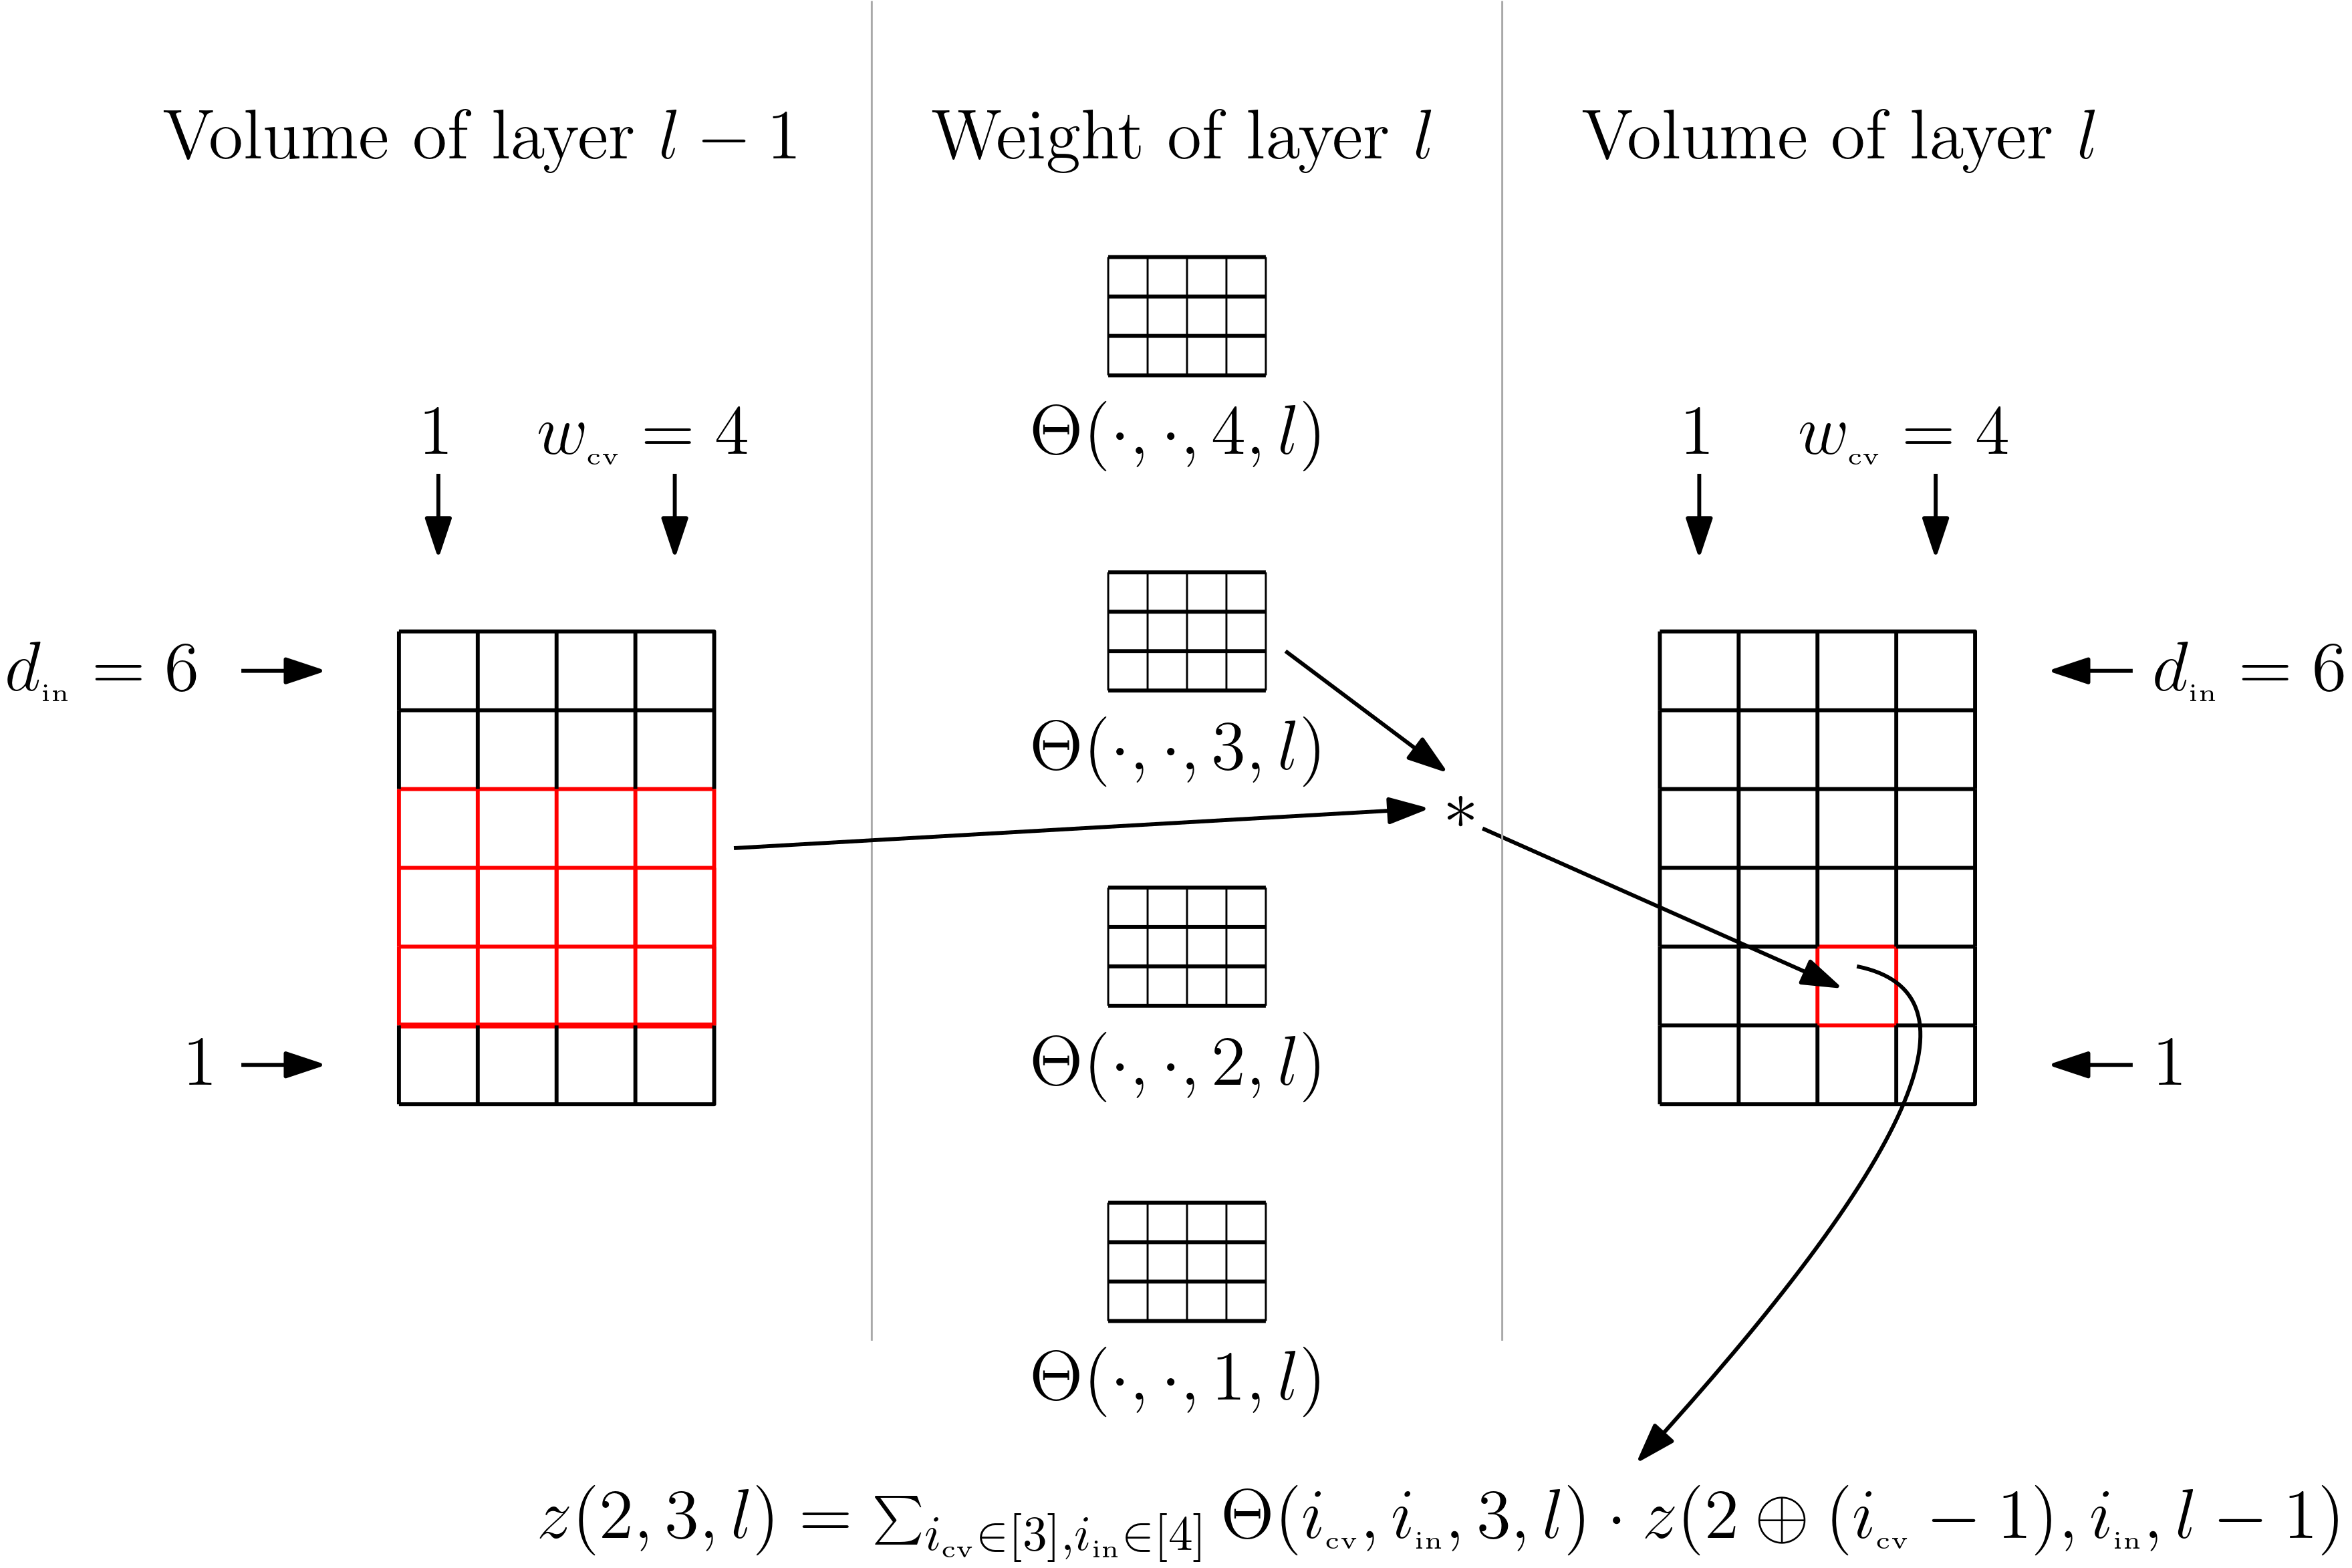
\includegraphics[scale=1]{figs/single-filter.png}
}
\end{figure}
\newpage
